\documentclass[12pt]{article}
\usepackage{graphicx}
\usepackage{gensymb}
\usepackage[none]{hyphenat}
\usepackage{graphicx}
\usepackage{listings}
\usepackage[english]{babel}
\usepackage{graphicx}
\usepackage{caption}
\usepackage{hyperref}
\usepackage{booktabs}
\usepackage{array}
\usepackage{amsmath}
\usepackage{listings}
\usepackage{multirow}
\usepackage{blindtext}
\usepackage{capt-of}
\usepackage{circuitikz}
\usepackage{./karnaugh-map}
\usetikzlibrary{shapes.geometric}
\title{Implementation of 4x1 mux in Arduino using Assembly}
\date{March 2023}
\author{Sai Harshith Kalithkar\\harshith.work@gmail.com\\FWC22118\\IIT Hyderabad-Future Wireless Communication Assignment}
\lstset{
	frame=single'
	breaklines=true
}
\newcommand{\mydet}[1]{\ensuremath{\begin{vmatrix}#1\end{vmatrix}}}
\providecommand{\brak}[1]{\ensuremath{\left(#1\right)}}
\providecommand{\norm}[1]{\left\lvert#1\right\rVert}
\newcommand{\solution}{\noindent \textbf{Solution: }}
\newcommand{\myvec}[1]{\ensuremath{\begin{pmatrix}#1\end{pmatrix}}}
\let\vec\mathbf

\begin{document}
\maketitle
\tableofcontents
\pagebreak

	 \section{Problem}
	 (GATE EC-2022)\\

Q.19. Consider the 2-bit multiplexer(MUX) shown in the figure.For output to be the XOR of R and S,the values for $ W,X,Y$ and $Z$ are ?\newline
\begin{figure}[h]
\begin{tikzpicture}
	\draw (0,-10) rectangle (3,-14);
	\draw (5,-10) rectangle (8,-14);
	\draw (-2,-15) -- (4,-15);
	\draw (-1,-15) -- (-1,-13.5);
	\draw (-1,-13.5) -- (0,-13.5);
	\draw (4,-15) -- (4,-13.5);
	\draw (4,-13.5) -- (5,-13.5);
	\draw (-1.5,-10.5) -- (0,-10.5);
	\draw (3,-10.5) -- (5,-10.5);
	\draw (-2,-15) node[above]{$12 KHz$} -- (-1.5,-15);
	\draw (8,-10.5) -- (10,-10.5);
	\draw (0.25,-10.5) node{$D_1$};
	\draw (5.25,-10.5) node{$D_2$};
	\draw (2.75,-10.5) node{$Q_1$};
	\draw (2.75,-13.5) node{$Q_1'$};
	\draw (7.75,-10.5) node{$Q_2$};
	\draw (7.75,-13.5) node{$Q_2'$};
	\draw (0.30,-13.5) node{$Clk$};
	\draw (5.30,-13.5) node{$Clk$};
	\node[and port] (a) at (-1.5,-10.5){};
	\draw (3,-13.5) -- (3.5,-13.5);
	\draw (3.5,-13.5) -- (3.5,-9.75);
	\draw (3.5,-9.75) -| (a.in 1);
	\draw (8,-13.5) -- (8.5,-13.5);
	\draw (8.5,-13.5) -- (8.5,-9.5);
	\draw (8.5,-9.5) -- (-3.5,-9.5);
	\draw (-3.5,-9.5) -- (-3.5,-10.78);
	\draw (-3.5,-10.78) -- (a.in 2);
\end{tikzpicture}

\caption{mux}
\label{fig:1}
\end{figure}
\begin{enumerate}
\item $W = 0, X = 0, Y = 1, Z = 1$
\item $W = 1, X = 0, Y = 1, Z = 0$
\item $W = 0, X = 1, Y = 1, Z = 0$
\item $W = 1, X = 1, Y = 0, Z = 0$
\end{enumerate}
\section{Introduction}
	The above diagram is a 4:1 multiplexer where $W, X, Y, Z$ are the inputs of the multiplexer and $A$ is the output of the multiplexer.$R , S$ are the select lines of the multiplexer,which means:\newline
\begin{enumerate}
\item For $R = 0,S = 0$,the first input line $W$ is selected.
\item For $R = 0,S = 1$,the second input line $X$ is selected.
\item For $R = 1,S = 0$,the third input line $Y$ is selected.
\item For $R = 1,S = 1$,the fourth input line $Z$ is selected.
\end{enumerate}
Therefore,the resultant output expression of the multiplexer is $R'S'W + R'SX + RS'Y + RSZ$.
\section{Components}
\begin{table}[h]
	\begin{tabular}{|p{3cm}|p{3cm}|p{3cm}|}
\hline                                        
	\textbf{Symbol} & \textbf{Values} & \textbf{Description} \\                                          
\hline                                 
	a & 3 & $AD=BC$ \\        
\hline                                    
	b & 4 & $AB$ \\    
\hline                      
	$\vec{e}_1$ & $\myvec{1\\0}$ & basis vector \\
\hline
\end{tabular}

\caption{contents}
\label{table 1}
\end{table}
	\pagebreak
\section{Hardware}
	\begin{enumerate}
\item Connect the COM of the seven-segment display to 5V and dot of the seven-segment to the ground.
\item Now connect any one of the pin of the seven-segment to pin no.2(digital).
\item Pin no.s 5,6,7,8 of the arduino should be initially connected to ground.
\item Now move pin no.s 5,6,7,8 accordingly and for the right combination the second pin of the arduino becomes high and the seven segement display glows.
\end{enumerate}
\begin{table}[h]
\begin{center}
	\begin{tabular}[h]{|c|c|c|c|}
\hline \multicolumn{2}{|c|}{INPUT} & \multicolumn{2}{|c|}{OUTPUT} \\
\hline $Q_1$ & $Q_2$ & $D_1$ & $D_2$ \\
\hline 0 & 0 & 1 & 0 \\
\hline 1 & 0 & 0 & 1 \\
\hline 0 & 1 & 0 & 0 \\
\hline
\end{tabular}

\end{center}
\caption{truth table}
\label{table 2}
\end{table}
The K-map for this truth table will be a two variable K-map and it will be as follows:
\begin{figure}[h]
	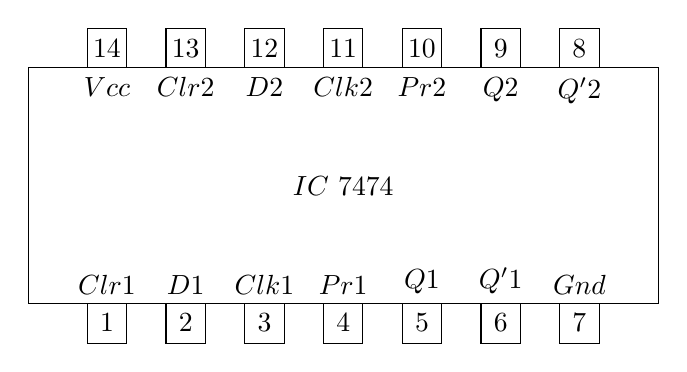
\begin{tikzpicture}                                           
	\draw (0,2) rectangle (8,5);                         
	\draw (4,3.5) node{$IC$ $7474$};                    
	\draw (0.75,2) rectangle (1.25,1.5);               
	\draw (1,2) node[below]{$1$};                        
	\draw (1,2) node[above]{$Clr1$};                     
	\draw (1.75,2) rectangle (2.25,1.5);                 
	\draw (2,2) node[below]{$2$};                      
	\draw (2,2) node[above]{$D1$};                        
	\draw (2.75,2) rectangle (3.25,1.5);                                                                        
	\draw (3,2) node[below]{$3$};                   
	\draw (3,2) node[above]{$Clk1$};                   
	\draw (3.75,2) rectangle (4.25,1.5);             
	\draw (4,2) node[below]{$4$};                 
	\draw (4,2) node[above]{$Pr1$};                      
	\draw (4.75,2) rectangle (5.25,1.5);                  
	\draw (5,2) node[below]{$5$};                        
	\draw (5,2) node[above]{$Q1$};                                                                               
	\draw (5.75,2) rectangle (6.25,1.5);                 
	\draw (6,2) node[below]{$6$};                        
	\draw (6,2) node[above]{$Q'1$};                      
	\draw (6.75,2) rectangle (7.25,1.5);               
	\draw (7,2) node[below]{$7$};                     
	\draw (7,2) node[above]{$Gnd$};                    
	\draw (0.75,5) rectangle (1.25,5.5);               
	\draw (1,5) node[above]{$14$};                      
	\draw (1,5) node[below]{$Vcc$};                    
	\draw (1.75,5) rectangle (2.25,5.5);                 
	\draw (2,5) node[above]{$13$};                       
	\draw (2,5) node[below]{$Clr2$};
                
		\draw (2.75,5) rectangle (3.25,5.5);               
		\draw (3,5) node[above]{$12$};                      
		\draw (3,5) node[below]{$D2$};                     
		\draw (3.75,5) rectangle (4.25,5.5);                
		\draw (4,5) node[above]{$11$};                       
		\draw (4,5) node[below]{$Clk2$};                    
		\draw (4.75,5) rectangle (5.25,5.5);               
		\draw (5,5) node[above]{$10$};
		\draw (5,5) node[below]{$Pr2$};                    
		\draw (5.75,5) rectangle (6.25,5.5);              
		\draw (6,5) node[above]{$9$};                       
		\draw (6,5) node[below]{$Q2$};                     
		\draw (6.75,5) rectangle (7.25,5.5);               
		\draw (7,5) node[above]{$8$};                      
		\draw (7,5) node[below]{$Q'2$};             
\end{tikzpicture}                                  

\caption{k-map}
\label{fig2}
\end{figure}

So,the resultant expression of A is $A = R'S + RS'$.
\pagebreak
\section{Software}

The Assembly code for the given circuit is \\ 
\lstinputlisting{code/assembly.asm}
\end{document}
